\chapter{Nasazení}

\indent

K testování a provozu webové aplikace jsem získál virtualizovaný server, ke kterému přistupuji pomocí SSH
\footnote{Program, který komunikuje zabezpečeným komunikačním protokolem. Používá TCP/IP.}.

\subsection*{Virtuální privátní server}

\indent

Jde o server běžící na virtualizovaném hardwaru a často se označuje zkratkou VSP.
Bývá poskytován hostingovými společnostmi, které svůj fyzický stroj nabízejí více klientům najednou.
Každému zákazníkovi vymezí prostor s vlastní instancí operačního systému, jednotlivými hostingovými službami
a vlastní konfigurací. Nevýhodu je sdílení fyzických prostředků, poněvadž při nedostatečném nastavení
může docházet k ovlivňování cizích VPS. Výhodou je naopak levnější pořízení ve srovnání celého fyzického serveru.

\section{Softwarové požadavky}

\indent

Aplikace běží na VPS s OS Ubuntu verze 15.10. Na veřejné adrese virtulního serveru
je dostupná RESTová webová služba Catcher, s níž může zvnějšku komunikovat libovolná aplikace,
která disponuje HTTP protokolem a dostupností běžného portu 80. Jako prostředník mezi klientskou aplikací
a uWSGI 2.0.12, jehož úkolem je udržovat Catchera, zde běží webový server Nginx 1.9.3.
Data se ukládají na databázový server MySQL verze 5.6.28.

\medskip

Pro běh aplikace byly stáhnuty všechny potřebné balíčky včetně pipu,
jenž slouží pro správu nesystémových knihoven v Pythonu. Detailní seznam všech zásvislostí obsahuje soubor
\texttt{README.md}, uložený v rodičovském adresáři projektu. Lepší správu souborů mi pak zajistil program Midnight Commander.

\begin{figure}[ht!]
\centering
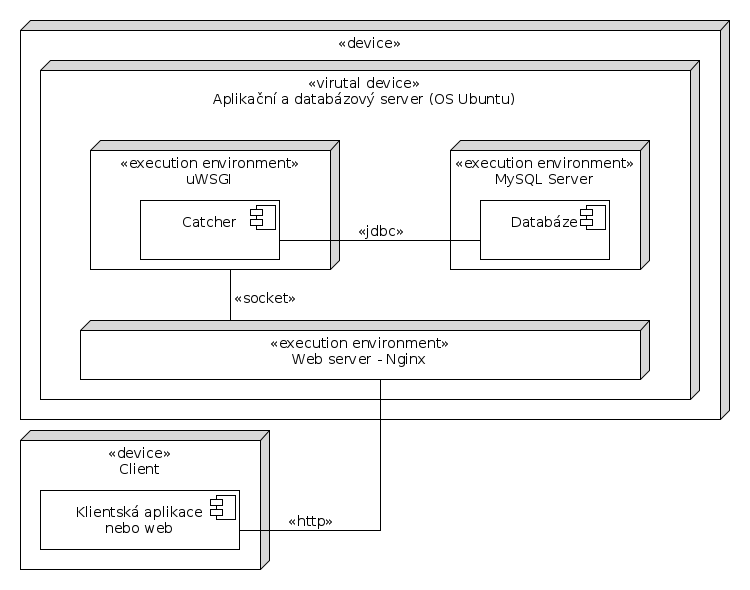
\includegraphics[width=130mm]{./images/diagram-nasazeni.png}
\caption{Diagram nasazení\label{overflow}}
\end{figure}

\section{uWSGI}

\indent

Aby bylo lépe pochopitelné zapojení uWSGI do celého procesu nasazení, popíšeme si jej trochu detailněji.

\medskip

Projekt uWSGI je malý program, který se stará o management procesu aplikace.
Funguje jako prostředník mezi aplikací a webovým serverem,
se kterými komunikuje vlastním uwsgi protokolem, respektive standartním WSGI
\footnote{WSGI je komunikační protokol mezi aplikací napsanou v Pythonu a webovým serverem.}.
Detaily komunikace jsou vidět na obrázku ~\ref{fig:uwsgi}.

\begin{figure}[ht!]
\centering
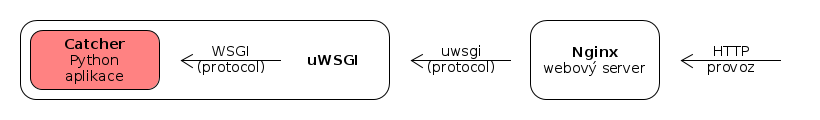
\includegraphics[width=135mm]{./images/uwsgi.png}
\caption{Komunikace mezi webovým serverem a aplikací v Pythonu \cite{uwsgi}.\label{overflow}}
\label{fig:uwsgi}
\end{figure}

%\label{fig:uwsgi}


% TODO: hezky diagram a povidani je na https://www.zdrojak.cz/clanky/produkcni-nasazeni-django-aplikaci-na-cherokee-pomoci-wsgi/ 

\subsection*{uWSGI úloha}

\indent

Spuštění webové aplikace provadím následujícím příkazem. Proces poslouchá na portu 8080 a po celou dobu běží na pozadí.

\begingroup
\fontsize{9.5pt}{11pt}\selectfont
\begin{verbatim}
$ uwsgi --socket localhost:8080 --wsgi-file ./restapi.py --callable api &
\end{verbatim}
\endgroup

\section{Konfigurace}

\subsection*{Konfigurační soubor}

\indent

Protože všechny moje zdrojové kódy byly zveřejněny v repozitáři na GitHubu, nebylo správné aby obsahovaly jakkákoliv hesla.
Pro tyto potřeby byl vytvořen konfigurační soubor, který mám zazálohovaný na vlastním cloudovém uložišti
a~pomocí programu wget si jej stahuju do daného adresáře vždy, když je změněn.
Tento konfigurační soubor obsahuje hesla k produkční a testovací databázi
nebo k emailovému účtu, který používám pro obnovu hesla uživatelů.

\subsection*{Databáze}

\indent

Pro přístup do databáze bylo potřeba vytvořit uživatele s právem zapisovat, číst a mazat.
Tento účet se nadále autentizuje heslem, které je uložené v konfiguračním souboru.
Příkazy pro vytvoření uživatele v SQL jsou následující:

\begingroup
\fontsize{9.5pt}{11pt}\selectfont
\begin{verbatim}
CREATE USER 'catcher-server'@'localhost' IDENTIFIED BY 'tajne_heslo';
GRANT SELECT, INSERT, UPDATE, DELETE
    ON catcher. * TO 'catcher-server'@'localhost';
\end{verbatim}
\endgroup

\subsection*{Nginx}

\indent

Protože disponuji pouze jednou veřejnou adresou na VPS, bylo potřeba webový server nakonfigurovat tak,
aby dokázal obsluhovat požadavky webové aplikace i požadavky
na zobrazení dokumentace. Konfigurace na serveru byla následující:

\subsubsection*{/etc/nginx/sites-enabled/catcher.conf}

\begingroup
\fontsize{9.5pt}{11pt}\selectfont
\begin{verbatim}
upstream catcher_uwsgi {
    # adresa a port, na které přeposílám požadavky pro Catchera
    server localhost:8080;
}

server {
    # číslo portu na ipv4
    listen       80;
    # číslo portu na ipv6
    listen       [::]:80;
    # jméno serveru
    server_name  catcher.zlutazimnice.cz *.catcher.zlutazimnice.cz;
    charset      utf-8;
    index        index.html;
    
    # maximální velikost uploadu
    client_max_body_size 75M;

    # dokumentace na catcher.zlutazimnice.cz
    location / {
        # adresář s obsahem webu
        root   /var/www/catcher;
    }

    # webová aplikace na catcher.zlutazimnice.cz/api
    location /api {
        include     uwsgi_params;
        # upstream pro spojení s uwsgi
        uwsgi_pass  catcher_uwsgi;
    }
}
\end{verbatim}
\endgroup

\medskip

Pro vývoj na svém počítači jsem použil trochu odlišnou konfiguraci, protože
jsem nemusel na jedné adrese provozovat dokumentaci i aplikaci.
V prvních fázích jsem dokonce ani Nginx používat nemusel, protože uWSGI umožňuje simulovat
chování webového serveru a jako prostředníka jsem jej tedy mohl vynechat.
Pro produkční nasazení ale není tento postup doporučen.

\section{Údržba}

\indent

Standartem pro větší aplikace by měl být monitorovací systém,
který sleduje zátěž jednotlivých komponent (webová aplikace, databáze, webový server atd.)
a~v~případě výpadku informuje administrátora sms zprávou nebo emailem.
Catcher však disponuje vlastností, že ještě nějakou dobu nebude nasazen do ostrého provozu
a~pro~tyto potřeby by měl stačit Cron\footnote{Jde o softwarového démona, který slouží
k~automatickému spouštění periodicky se opakujících příkazů a procesů.}
, který by v pravidelných intervalech \uv{oťukával} aplikaci a~stanovil, zda korektně běží.
Kromě toho může pravidelně zálohovat databázi příkazem \pythoninline{mysqldump}\footnote{Zde popíšu mysqldump.}.
V případě výpadku by tak stačilo aplikaci opravit a nahrát poslední zálohu.
Catcher aktuálně disponuje pouze manuálním zálohováním databáze.

% TODO: Dopsat, co dela mysqldump!!

% TODO: IDEA: Pouzit nasledujici:

%\section{Co by šlo udělat lépe}
%Během vývoje jsem se setkal se zajímavými nástroji, na které v tomto projektu nezbyla kapacita. Jejih použití by přineslo několik zlepšení, proto jsem se rozhodl je zde uvést:
%list:
%Virtualenv, Codevoc, Travis CI
%IDEA: Lze se zminit o testovani a prubezne integraci. Napriklad napsat, ze mame zajem v budoucnu pouzivat Codevoc (mozna spis testovani) nebo Travis CI.